\documentclass[a4paper,11pt]{article}
\usepackage[T1]{fontenc}
\usepackage[utf8]{inputenc}
\usepackage{lmodern}
\usepackage{graphicx}
\usepackage{float}

\title{Data Mining Coursework}
\author{Junaid Ali Rasheed}


\begin{document}

\maketitle

\begin{abstract}
\end{abstract}

\section{Introduction}
We have been provided with a dataset which contains information about customers
who were targets of direct marketing campaigns of a Portuguese banking institution.
Our task is to develop models on this dataset to determine whether a customer
will make a term deposit or not. We will use equal and unequal costs to develop
the model.

\section{Data Exploration}

The dataset was provided in the ARFF file format which can be used with Weka. Opening
the file in a text editor gives us a brief description of each attribute in the dataset.
An exploration of the dataset using a text editor and the Weka Explorer interface
reveals the following...

\begin{itemize}
  \item{The number of clients (people who were contacted by the banking institution) in
  the dataset is 36,188.}
  \item{31,981 clients did not make a term deposit, 4188 clients did make a term deposit.}
  \item{88.4\% of clients did not make a term deposit. This is the accuracy of the default classifier.} 
  \item{There are 16 attributes (excluding the output attribute, 'termDeposit').}
  \item{Reducing the number of attributes may be beneficial to avoid overfitting.}
  \item{There are no missing values. However, some attributes have an 'unknown' value.}
  \begin{itemize}
    \item{Job: Only 223 clients had an unknown job.}
    \item{Education: Only 1480 clients had an unknown education.}
    \item{Contact: 10417 clients were contacted by unknown means. The histogram (see Figure ~\ref{fig:contactHistogram}) shows
    that clients contacted by a cellular device (23416) were more likely to make a deposit
    compared to clients contacted by telephone (2336), so it would have been useful to know how
    all clients were contacted}
    \item{Previous campaign outcome: The value of this is 'unknown' for 29621 clients. This abnormally
    large number may be due to the fact that 29616 clients were never contacted for previous campaigns.}
  \end{itemize}
  \item{Viewing the histograms for each variable showed that clients who had defaulted
  would never make a term deposit}
  \item{Some attributes distribution of values were quite imbalanced.}
  \begin{itemize}
      \item{Balance: Strongly skewed distribution. Most clients had a low/negative balance.}
      \item{Month: 25800 clients were contacted in May, June, July, and August.}
      \item{Previous days: 29712 clients had a value of -1, meaning they were not previously contacted}
      \item{Previous: 29616 clients were not contacted for previous marketing campaigns.}
      \item{Job: There are 13 values but 7 of them include only 7267 clients}
  \end{itemize}
  \item{Two-dimensional scatter plots do not show any strong class separation for any of the attributes.
  From this, we can infer that several attributes will be needed to determine whether a client will
  make a term deposit or not.}
\end{itemize}

\begin{figure}[H]
  \centering
  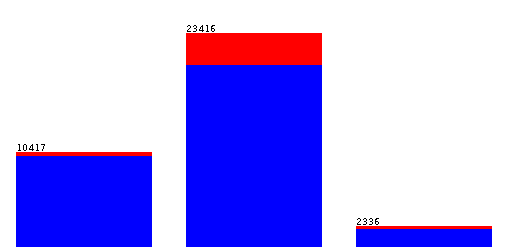
\includegraphics[width=0.8\textwidth]{pictures/contactHistogram.png}
  \caption{Histogram of the contact attribute}
  \label{fig:contactHistogram}
\end{figure}

\section{Data Preprocessing}

\section{Classification Models}

\section{Conclusion}


\end{document}
